When it comes to blackbox attacks, two existing approaches are evaluated: the Transfer based approach and the Boundary attack. In this section, results are only presented, but not discussed. The discussion is left for Section \ref{sec:discussion}.

In the transfer based approach, as described in Section \ref{sec:transfer-based}, the goal is to train a substitute network that will learn similar decision boundaries for every class as the targeted network. That implies that total number of possible classes should be the same, but an architecture of the substitute network may be different.

In my first attempt, I tried to use the ResNet-50 architecture as a substitute network, but the experiment failed due to memory consumption when jacobian augmentation of the dataset is performed. 
In my second attempt, I tried to use somewhat simpler architecture. The substitute network used the VGG16 architecture, but the experiment again failed due to the same reason.

In my third attempt?!

Finally, since the goal is to have similar boundaries as the targeted neural network, those boundaries could be obtained by just querying the targeted neural network and then learning the substitute neural network based on the results of queries. That skips a step of the jacobian augmentation of the dataset though. 

To get information about boundaries of the targeted neural network,  I take 1000 samples that are previously unseen to targeted neural network, obtain labels for those samples and train the substitute neural network based on those results. TODO: Distribution of ages in those 1000 samples

Which neural network is used as a substitute?

Next, I take random 100 samples that are yet unseen by both networks and evaluate MAE of the targeted neural network and the substitute network on those 100 images. Then I craft adversarial samples for the substitute neural network using those 100 images. Target labels for adversarial samples are set in the same manner as in whitebox attacks, i.e. label 90 if a person is under 50 years old and label 10 if a person is over 50 years old. 

Finally, I evaluate MAE of the targeted neural network and the substitute network on the 100 adversarial samples crafted in the previous step.

Results are presented in Tables \ref{table:bbox-fgsm-resnet} and \ref{table:bbox-cw-resnet}.

\begin{table}[]
\begin{tabular}{|c|c|c|c|c|}
\hline
 & \multicolumn{2}{c|}{Clean Samples} & \multicolumn{2}{c|}{Adversarial samples} \\ \hline
Target model id & Blackbox MAE & Substitute MAE & Blackbox MAE & Substitute MAE \\ \hline
1 & 6.21 & 14.17 & 6.61 & 14.20 \\ \hline
2 & 8.61 & 13.20  &  8.17 & 13.39  \\ \hline
3 & TODO & TODO  & TODO & TODO  \\ \hline
4 & TODO & TODO & TODO & TODO \\ \hline
\end{tabular}
\caption{Results using the ResNet-50 architecture for the substitute network and FGSM attack for crafting adversarial samples for it}
\label{table:bbox-fgsm-resnet}
\end{table}


\begin{table}[]
\begin{tabular}{|c|c|c|c|c|}
\hline
 & \multicolumn{2}{c|}{Clean Samples} & \multicolumn{2}{c|}{Adversarial samples} \\ \hline
Target model id & Blackbox MAE & Substitute MAE & Blackbox MAE & Substitute MAE \\ \hline
1 & 6.21 & 15.92 & 6.10 & 15.93 \\ \hline
2 &  TODO & TODO  & TODO &  \\ \hline
3 &  TODO & TODO  & TODO &  \\ \hline
4 &  TODO & TODO  & TODO &  \\ \hline
\end{tabular}
\caption{Results using the ResNet-50 architecture for the substitute network and CW attack for crafting adversarial samples for it}
\label{table:bbox-cw-resnet}
\end{table}

Regarding the boundary attack, it's hard to do any quantitative analysis because the attack, as described in Section \ref{sec:boundary-attack}, is fundamentally different that the transfer based approach. Instead, I generate several samples and discuss them. One sample can be seen in Figure \ref{fig:trump-adv} and the corresponding results in Figure \ref{fig:trump-softmax}. TODO: ADD reference to other images. The other samples can be found in Appendix. 
\begin{figure}
\begin{subfigure}{.5\textwidth}
  \centering%
  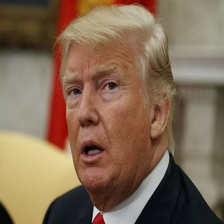
\includegraphics[height=5cm, width=\linewidth, keepaspectratio]{image0.jpg}
  \caption{The starting image}
\end{subfigure}
\begin{subfigure}{.5\textwidth}
  \centering
  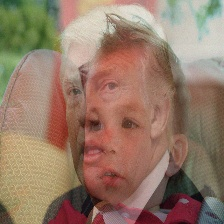
\includegraphics[height=5cm, width=\linewidth, keepaspectratio]{image1000.jpg}
  \caption{1000 queries}
\end{subfigure}

\begin{subfigure}{.5\textwidth}
  \centering
  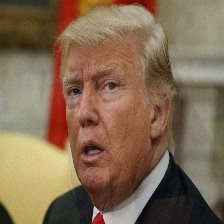
\includegraphics[height=5cm, width=\linewidth, keepaspectratio]{image2000.jpg}
  \caption{2000 queries}
\end{subfigure}
\begin{subfigure}{.5\textwidth}
  \centering
  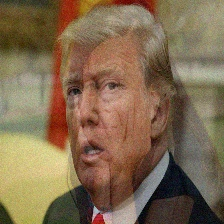
\includegraphics[height=5cm, width=\linewidth, keepaspectratio]{image4000.jpg}
  \caption{4000 queries}
\end{subfigure}

\begin{subfigure}{.5\textwidth}
  \centering
  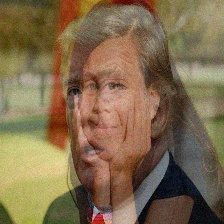
\includegraphics[height=5cm, width=\linewidth, keepaspectratio]{image8000.jpg}
  \caption{8000 queries}
\end{subfigure}
\begin{subfigure}{.5\textwidth}
  \centering
  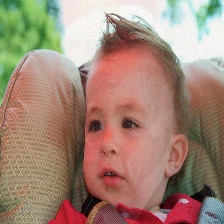
\includegraphics[height=5cm, width=\linewidth, keepaspectratio]{image12000.jpg}
  \caption{12000 queries}
\end{subfigure}

\begin{subfigure}{.5\textwidth}
  \centering
  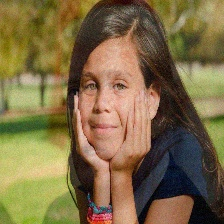
\includegraphics[height=5cm, width=\linewidth, keepaspectratio]{image16000.jpg}
  \caption{16000 queries}
\end{subfigure}
\begin{subfigure}{.5\textwidth}
  \centering
  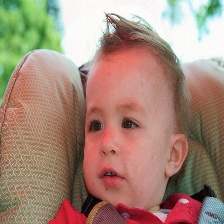
\includegraphics[height=5cm, width=\linewidth, keepaspectratio]{final_adversarial.jpg}
  \caption{Final adversarial sample}
\end{subfigure}
\caption{Although an adversary is changing the image, the blackbox classifier is not changing the prediction (68 years old)}
\label{fig:trump-adv}
\end{figure}

\begin{figure}
\begin{subfigure}{.5\textwidth}
  \centering
  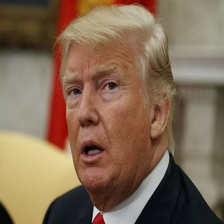
\includegraphics[height=5cm, width=\linewidth, keepaspectratio]{image0.jpg}
  \caption{Starting image}
\end{subfigure}
\begin{subfigure}{.5\textwidth}
  \centering
  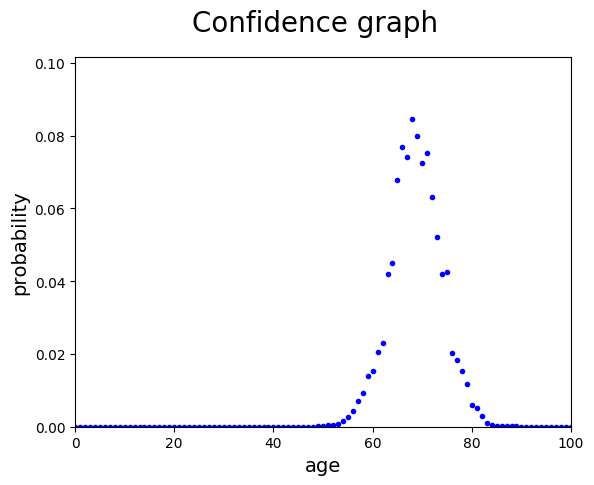
\includegraphics[height=5cm, width=\linewidth, keepaspectratio]{softmaxbenign.png}
  \caption{Predictions for the starting image}
\end{subfigure}
\caption{Starting image and the corresponding prediction}
\label{fig:starting-image-softmax}
\end{figure}

\begin{figure}
\begin{subfigure}{.5\textwidth}
  \centering
  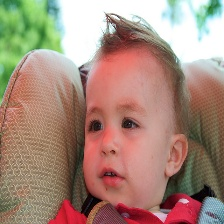
\includegraphics[height=5cm, width=\linewidth, keepaspectratio]{source_image.jpg}
  \caption{The targeted image}
\end{subfigure}
\begin{subfigure}{.5\textwidth}
  \centering
  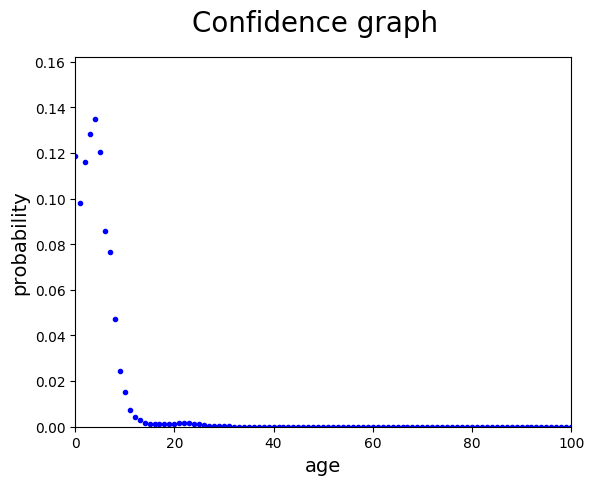
\includegraphics[height=5cm, width=\linewidth, keepaspectratio]{softmaxsource_image.png}
  \caption{Predictions for the targeted image}
\end{subfigure}

\caption{Targeted image and the corresponding predictions}
\label{fig:targeted-image-softmax}
\end{figure}

\begin{figure}

\begin{subfigure}{.5\textwidth}
  \centering%
  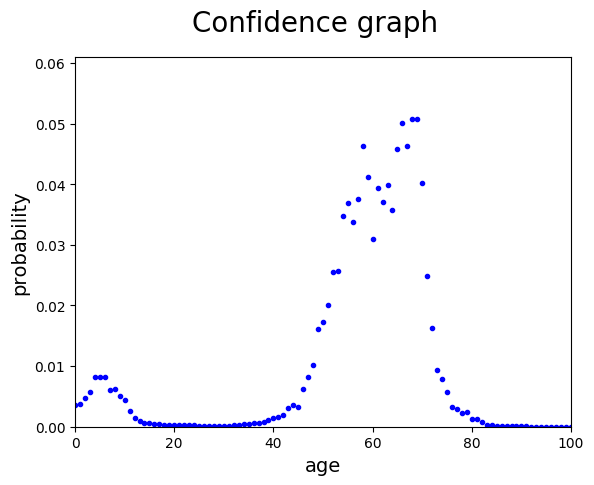
\includegraphics[height=5cm, width=\linewidth, keepaspectratio]{softmax3000.png}
  \caption{3000 queries}
\end{subfigure}
\begin{subfigure}{.5\textwidth}
  \centering%
  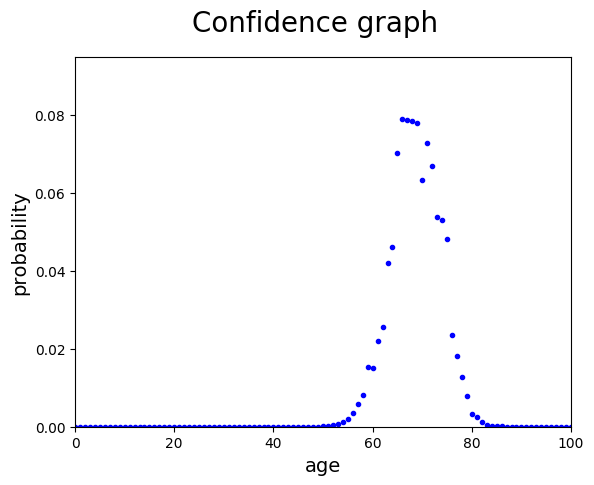
\includegraphics[height=5cm, width=\linewidth, keepaspectratio]{softmax4000.png}
  \caption{4000 queries}
\end{subfigure}


\begin{subfigure}{.5\textwidth}
  \centering%
  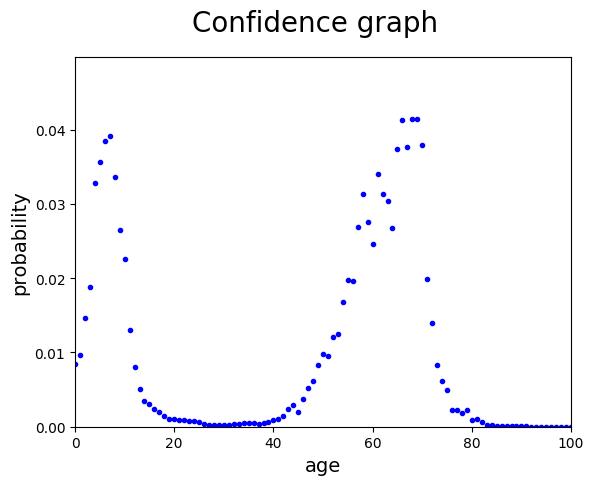
\includegraphics[height=5cm, width=\linewidth, keepaspectratio]{softmax8000.png}
  \caption{8000 queries}
\end{subfigure}
\begin{subfigure}{.5\textwidth}
  \centering%
  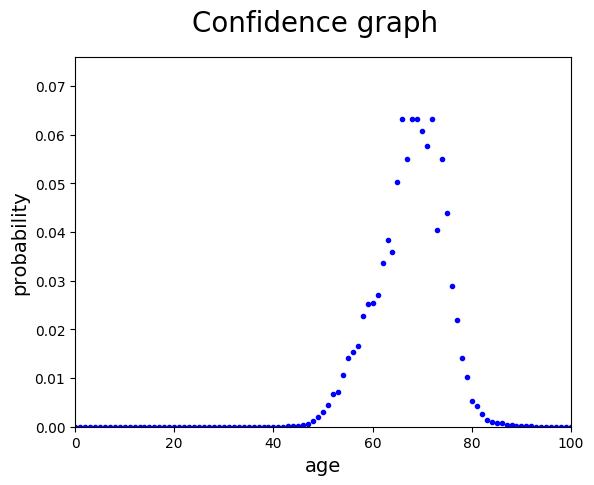
\includegraphics[height=5cm, width=\linewidth, keepaspectratio]{softmaxadversarial.png}
  \caption{The final adversarial sample (77 000 queries)}
\end{subfigure}

\caption{Predictions of the blackbox classifier for images corresponding to Figure \ref{fig:trump-adv}. In all the graphs, age 68 is predicted with the maximum probability.}
\label{fig:trump-softmax}
\end{figure}


